\documentclass[12pt]{article}

\usepackage{listings}
\usepackage[most]{tcolorbox}
\usepackage{inconsolata}
\usepackage{pslatex}
\usepackage{units}
\usepackage{graphicx}
\usepackage{longtable}
\usepackage{siunitx}

\newtcblisting[auto counter]{codelisting}[2][]{sharp corners, 
	fonttitle=\bfseries, colframe=gray, listing only, 
	listing options={basicstyle=\ttfamily,language=python}, 
	title=Listing \thetcbcounter: #2, #1}

\oddsidemargin  0mm
\evensidemargin 0mm
\pagestyle{plain}
\textheight  261mm
\topmargin  -10mm
\textwidth   16cm

\newcommand{\E}{\mathbb{E}}
\title{Sports Match Predictor}
\author{\makebox[.9\textwidth]{Rui Carapinha} \and Witold Paluszynski\\Wroclaw Univesity of Technology\\Politechnika Wroclawska}

\date{23/01/2019}

\begin{document}
\pdfpageheight   29.7cm
\pdfpagewidth    21cm
 
\maketitle

% 1 - Introduction
\section{Introduction}

My project is Sports Match Predictor, the goal of the project is to predict the results of a choosen match with a rather good certainty. The program I used for this project was Python 3 and I also used a database from previous seasons. In this project I tried to build a model that predicts the outcome of each match - win, draw or defeat based on a Poisson distribution.

% 2 - Software
\subsection{Coding}
In this part of the report I'll explain, part by part, how the code works. First step is to to take care of the data and analyzing it in a proper way so that I can handle it easily. So, I started by listing all the teams in the database:

\begin{codelisting}{List All Teams}
def ListAllTeams():
	csv_file = csv.reader(open('E0.csv'))
	next(csv_file)

	teams_l = list()
	i = 0
	for game in csv_file:
		if game[2] in teams_l:
			i = i
		else:
			teams_l.insert(i, game[2])
			i = i+1
	return teams_l
\end{codelisting}

This code goes line by line and then checks if the team is already in the list. If the team is in the list it simply ignores  it and goes to the next line. If it isn't in the list, it adds to the list and passes to the next line.

The next step was to list all the stats of the teams (Number of home games, number of away games, goals conceded and scored in home games, goals conceded and scored in away games) this is will be used to create some sorte of team experience (this team experience will be based on their attack and defense in home games and their attack and defense in away games). The code is the following:

\begin{codelisting}{Team Stats - Part 1}
def ListStats(teams):
	ForGoals_l = list()
	AwayGoals_l = list()

	home_team_a = list()
	home_team_d = list()
	away_team_a = list()
	away_team_d = list()

	homegames_l = list()
	awaygames_l = list()
	avg_for_home_goals_l = list()
	avg_against_home_goals_l = list()
	avg_for_away_goals_l = list()
	avg_against_away_goals_l = list()

	for team_c in teams:
		csv_file = csv.reader(open('E0.csv'))
		next(csv_file)

		HomeForGoals = 0
		HomeAgainstGoals = 0
		AwayForGoals = 0
		AwayAgainstGoals = 0
		ForGoals = 0
		AgainstGoals = 0
		HomeGames = 0
		AwayGames = 0

		for fixt in csv_file:	
			if (team_c == fixt[2]):
			       HomeGames += 1
			       HomeForGoals+=int(fixt[4])
			       HomeAgainstGoals+=int(fixt[5])
			elif (team_c == fixt[3]):
			       AwayGames += 1
			       AwayForGoals+=int(fixt[5])
			       AwayAgainstGoals+=int(fixt[4])
\end{codelisting}

\begin{codelisting}{Team Stats - Part 2}
ind = teams.index(team_c)

homegames_l.insert(ind, HomeGames)
awaygames_l.insert(ind, AwayGames)

avg_for_home_goals_l.insert(ind,HomeForGoals/HomeGames)
avg_against_home_goals_l.insert(ind,HomeAgainstGoals/HomeGames)
avg_for_away_goals_l.insert(ind,AwayForGoals/AwayGames)
avg_against_away_goals_l.insert(ind,AwayAgainstGoals/AwayGames)

home_team_a.insert(ind, HomeForGoals/HomeGames)
home_team_d.insert(ind, HomeAgainstGoals/HomeGames)
away_team_a.insert(ind, AwayForGoals/AwayGames)
away_team_d.insert(ind, AwayAgainstGoals/AwayGames)

return home_team_a,home_team_d,away_team_a,away_team_d,
avg_for_home_goals_l,avg_for_away_goals_l
\end{codelisting}

The next part of the code, I calculate the team experience. The code is the following:

\begin{codelisting}{Team Experience}
All_teams = ListAllTeams()

HomeTeam_A, HomeTeam_D, AwayTeam_A, AwayTeam_D, 
AvgForHomeGoals, AvgForAwayGoals = ListStats(All_teams)
	
HomeExp = list()
AwayExp = list()

k = 0

while k < len(All_teams):
	AFHG = float(AvgForHomeGoals[k])
	AFAG = float(AvgForAwayGoals[k])


	HomeExp.insert(k,AFHG*float(HomeTeam_A[k])
*float(HomeTeam_D[k]))
	AwayExp.insert(k,AFAG*float(AwayTeam_A[k])
*float(AwayTeam_D[k]))
	k += 1
\end{codelisting}

This code calculates the team experience based on the variables taken from the above function and in the average of goals scored at home and away of home. The last part of the code is the following, this part of the code will ask the user to input the teams we want to predict the result and calculate the probabilities of home win, away win and draw based on the Poisson distribution. The code is the following:

\begin{codelisting}{Final Part of the Code}
j = 0
while j < len(All_teams):
	print(str(j) + " - "+ All_teams[j])
	j += 1
th_id = int(input("Choose Home Team -> "))
ta_id = int(input("Choose Away Team -> "))
csv_file = csv.reader(open('E0.csv'))
next(csv_file)
home_win_prob = 0
draw_prob = 0
away_win_prob = 0
for row in csv_file:
     if row[2] == All_teams[th_id]:
          if row[3] == All_teams[ta_id]:
               HomeG = row[4]
               AwayG = row[5]
               for i in range(10):
                    for j in range(10):
                         prob = poisson(i, HomeExp[th_id]) 
* poisson(j, AwayExp[ta_id])
                         if i > j:
                              home_win_prob += prob
                         elif i == j:
                              draw_prob += prob
                         elif i < j:
                              away_win_prob += prob					
               print("Home Win Probability: " 
+ str(home_win_prob))
               print("Away Win Probability: " 
+ str(away_win_prob))
               print("Draw Win Probability: " 
+ str(draw_prob))
               if (draw_prob > away_win_prob):
                    if (draw_prob > home_win_prob):
                         print("Draw")
               if (away_win_prob > home_win_prob):
                    print("Away Team Win")
               elif (away_win_prob < home_win_prob):
                    print("Home Team Win")
               print("Last Real Result: " + HomeG + " - " 
+ AwayG)

               break
\end{codelisting}

% 3 - Results
\section{Development}
In this part of the report I will explain the development I made through these months of the project. First, I splited the project in several objectives. They were the following:
\begin{itemize}
	\item Searching and studying the database of football
	\item Make prediction algorithm
	\item Create small interface
\end{itemize}

To make sure my algorithm is trustworthy, I tried to predict this season last three fixtures results using my algorithm. The results I had were the following:

\begin{figure}[!h]
	\center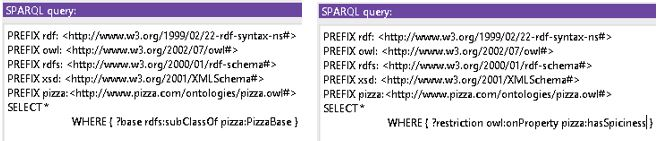
\includegraphics[width=0.6\textwidth]{Capture.jpg}
	\caption{Results}
\end{figure}

We should note that the English Premier League is one of the most unpredictable leagues of the world, every fixture there's almost always a big surprise (like a small team beating one of the best teams), for example, last fixture Newcastle (17th position in the league table) won against Manchester City (2nd position in the league table). As we can see in, in 28 matches my algorithm got 15 correct results, I achieved a 53.6 percent accuracy. This is still a bit low, we will need to improve this if we want to trust in this algorithm for betting purposes but it's a good start. 

\newpage
\section{Conclusion}

In conclusion the project was quite interesting because I as able to apply coding and mathematical knowledge to solve a problem that I like, using a database of a sports I love. In the beggining I wasn't sure if the Poisson implementation will work as a match prediction algorithm but I found the results quite nice. Neverthless, this project was a great experience because I never experienced to make a project with Python. The results of my project reflect a solid first effort in prediction match outcomes in football. This project can be improved by analyzing better the data (maybe doing some classification) and by studying more the predicition algorithm and also by implementing some machine learning techniques.

\section{References}
\begin{thebibliography}{} 
\bibitem{website} 
Database,
\\\texttt{http://www.football-data.co.uk}

\bibitem{website} 
Online Betting Guide,
\\\texttt{http://www.bestbettingonline.com/beginner}

\bibitem{website} 
Poisson Distribution in Football Betting Market  ,
\\\texttt{https://tolstoy.newcastle.edu.au/R/e8/help/att-6544/dixoncoles97.pdf}

\bibitem{website} 
Betting,
\\\texttt{http://www.bestbettingonline.com/strategy/create-model}

\end{thebibliography}

\end{document}